\documentclass{article}

\usepackage{fancyhdr}
\usepackage{extramarks}
\usepackage{amsmath,amssymb,mathrsfs}
\usepackage{amsthm}
\usepackage{amsfonts}
\usepackage{parskip}
\usepackage[version=3]{mhchem} 
\usepackage{fixltx2e}
\usepackage{refcount}
\usepackage{siunitx}
\usepackage{lastpage}
\usepackage{textcomp}
\usepackage{xfrac}
\usepackage{lmodern}
\usepackage{cool}
\usepackage{cancel}
\usepackage{microtype}
\usepackage{gensymb}
\usepackage{enumerate}
\usepackage{float}
\usepackage{bm}
\usepackage{csquotes}
\usepackage{mathtools}
\usepackage{mcode}

\usepackage[hidelinks]{hyperref}

\DeclarePairedDelimiter\bra{\langle}{\rvert}
\DeclarePairedDelimiter\ket{\lvert}{\rangle}
\DeclarePairedDelimiterX\braket[2]{\langle}{\rangle}{#1 \delimsize\vert #2}








%
% Basic Document Settings
%

\topmargin=-0.45in
\evensidemargin=0in
\oddsidemargin=0in
\textwidth=6.5in
\textheight=9.0in
\headsep=0.25in

\linespread{1.1}

\clubpenalty = 10000
\widowpenalty = 10000

\pagestyle{fancy}
\lhead{\hmwkAuthorName}
\chead{\hmwkClass\ \textemdash\ \hmwkTitle}
\rhead{\firstxmark}
\lfoot{\lastxmark}
\cfoot{ASV\twodigits{\thepage}\ of \twodigits{\getpagerefnumber{LastPage}}}

\renewcommand\headrulewidth{0.4pt}
\renewcommand\footrulewidth{0.4pt}

\setlength\parindent{0pt}
\setlength\parskip{1.2ex}





%
% Create Problem Sections
%

\newcommand{\enterProblemHeader}[1]{
    \nobreak\extramarks{}{Problem \arabic{#1} continued on next 
page\ldots}\nobreak{}
    \nobreak\extramarks{Problem \arabic{#1} (continued)}{Problem \arabic{#1} 
continued on next page\ldots}\nobreak{}
}

\newcommand{\exitProblemHeader}[1]{
    \nobreak\extramarks{Problem \arabic{#1} (continued)}{Problem \arabic{#1} 
continued on next page\ldots}\nobreak{}
    \stepcounter{#1}
    \nobreak\extramarks{Problem \arabic{#1}}{}\nobreak{}
    
}

\setcounter{secnumdepth}{0}
\newcounter{partCounter}
\newcounter{homeworkProblemCounter}
\setcounter{homeworkProblemCounter}{1}
\nobreak\extramarks{Problem \arabic{homeworkProblemCounter}}{}\nobreak{}

%
% Homework Problem Environment
%
% This environment takes an optional argument. When given, it will adjust the
% problem counter. This is useful for when the problems given for your
% assignment aren't sequential. See the last 3 problems of this template for an
% example.
%
\newenvironment{homeworkProblem}[1][-1]{
    \ifnum#1>0
	\setcounter{homeworkProblemCounter}{#1}
    \fi
%     \section{Problem \arabic{homeworkProblemCounter}}
    \setcounter{partCounter}{1}
    \enterProblemHeader{homeworkProblemCounter}
}{
    \exitProblemHeader{homeworkProblemCounter}
    \pagebreak

}

%
% Homework Details
%   - Title
%   - Due date
%   - Class
%   - Instructor
%   - Author
%

\newcommand{\hmwkTitle}{Homework\ \# 03}
\newcommand{\hmwkDueDate}{18 October 2016}
\newcommand{\hmwkClass}{NE 255}
\newcommand{\hmwkClassInstructor}{Professor Rachel Slaybaugh}
\newcommand{\hmwkAuthorName}{Andrew S Voyles}

%
% Title Page
%

\title{
%     \vspace{2in}
    \textmd{\textbf{\hmwkClass:\ \hmwkTitle}}\\
    \normalsize\vspace{0.1in}\small{Due\ \hmwkDueDate}\\
    \vspace{0.1in}\large{\textit{\hmwkClassInstructor}}
}

\author{\textbf{\hmwkAuthorName}}
\date{}

\renewcommand{\part}[1]{\textbf{\large Part 
\Alph{partCounter}}\stepcounter{partCounter}\\}

%
% Various Helper Commands
%

% Useful for algorithms
\newcommand{\alg}[1]{\textsc{\bfseries \footnotesize #1}}

% For derivatives
\newcommand{\deriv}[1]{\frac{\mathrm{d}}{\mathrm{d}x} (#1)}

% For partial derivatives
\newcommand{\simplepderiv}[2]{\frac{\partial}{\partial #1} (#2)}

% Integral dx
\newcommand{\dx}{\mathrm{d}x}

% Alias for the Solution section header
\newcommand{\solution}{\textbf{\large Solution}}

% One sentence of lorem ipsum text
\newcommand{\shortlipsum}{Lorem ipsum dolor sit amet, consectetuer adipiscing 
elit.}

% Pad zeroes for footer numbering
\newcommand\twodigits[1]{%
  \ifnum#1<10 0#1\else #1\fi
}

% Consistant figure references
\newcommand{\figref}[1]{Figure~\ref{#1}}

% Define partial derivative alias
\newcommand{\partialder}[2]{\dfrac{\partial #1}{\partial #2}}

% Volume symbol
\newcommand{\volume}{\mathop{\ooalign{\hfil$V$\hfil\cr\kern0.08em--\hfil\cr}}\nolimits}

% Area symbol
\newcommand{\area}{\mathop{\ooalign{\hfil$A$\hfil\cr\kern0.08em--\hfil\cr}}\nolimits}

% Sin and Cos with auto-parentheses 
\newcommand{\sinp}[1]{\sin{\left( #1\right)}}
\newcommand{\cosp}[1]{\cos{\left( #1\right)}}
\newcommand{\expp}[1]{\exp{\left( #1\right)}}
\newcommand{\sinhp}[1]{\sinh{\left( #1\right)}}
\newcommand{\lnp}[1]{\ln{\left( #1\right)}}
\newcommand{\pp}[1]{\left( #1\right)}
\newcommand{\sci}[2]{ #1 \cdot 10^{#2}\ }
\newcommand{\angstrom}{\mbox{\normalfont\AA}}
\newcommand{\norm}[1]{\lVert #1 \rVert}






% math syntax
\newcommand{\nth}{n\ensuremath{^{\text{th}}} }
\newcommand{\ve}[1]{\ensuremath{\mathbf{#1}}}
\newcommand{\Macro}{\ensuremath{\Sigma}}
\newcommand{\rvec}{\ensuremath{\vec{r}}}
\newcommand{\xvec}{\ensuremath{\vec{x}}}
\newcommand{\omvec}{\ensuremath{\hat{\Omega}}}
\newcommand{\vOmega}{\ensuremath{\hat{\Omega}}}


% Make vectors use boldface
\renewcommand{\vec}[1]{\mathbf{#1}}


% Consistant matrix notation
\newcommand{\matr}[1]{\mathbf{#1}} % undergraduate algebra version
% \newcommand{\matr}[1]{#1}          % pure math version
% \newcommand{\matr}[1]{\boldsymbol{#1}}     % ISO complying version


\makeatletter
% Make common definition of mean
\newcommand*\mean[1]{\overline{#1\raisebox{3mm}{}}}

\makeatother






\begin{document}

\maketitle
\thispagestyle{fancy}





\section{Problem 1}

\begin{homeworkProblem}

 (20 points)  Derive the 1st order form of $SP_5$ with isotropic source and vacuum boundary
conditions.




\subsection{Solution}
    
 XXXXXXXXXXXXXXXXXX
    

\end{homeworkProblem}


\section{Problem 2}

\begin{homeworkProblem}

Consider the integral

\begin{equation}
\int_{4\pi} d\omvec \left|\omvec\right|
\end{equation}

The LQ$_N$ quadrature set is given in \autoref{fig:LQquad}. Recall that $\mu_i = \eta_i = \xi_i$ for a given level, $i$.

\begin{figure}[H]
 \centering
 \includegraphics{./homework3-cropped.pdf}
 % homework3-cropped.pdf: 252x337 pixel, 72dpi, 8.89x11.89 cm, bb=0 0 252 337
 \caption{LQ$_n$ quadrature}
 \label{fig:LQquad}
\end{figure}


\begin{enumerate}[(a)] 

\item  (5 points)  Use the $S_4$ LQ$_N$ quadrature set to execute this integral.





\subsection{Solution}
    
  XXXXXXXXXXXXXXXXXXXXXX
 
   
\item    (10 points) Repeat it with $S_6$. What do you observe?




\subsection{Solution}
    
  XXXXXXXXXXXXXXXXXX
   
   \item (10 points) Write a short code to execute this integration (and higher orders if
you'd like). Try a few different functions. Turn in the code and the evaluation of
these functions. Include comments on what you observe.



\subsection{Solution}
    
  XXXXXXXXXXXXXXXXX


\end{enumerate}

\end{homeworkProblem}


\section{Problem 3}

\begin{homeworkProblem}




\begin{enumerate}[(a)] 

\item (5 points) Briefly compare the diffusion equation, deterministic methods, and monte
carlo methods in terms of complexity, accuracy, run time, and range of applicability.




\subsection{Solution}

XXXXXXXXXXXXXXXXXXXXXXXX
 
   
\item  (5 points) Given what you've learned about deterministic methods so far, discuss
strengths and weaknesses.




\subsection{Solution}

   XXXXXXXXXXXXXXXXXXXXXXXXXXXXx
   

\end{enumerate}

\end{homeworkProblem}



\section{Problem 4}

\begin{homeworkProblem}

Write a function that generates the associated Legendre Polynomials:

\begin{equation}
P_\ell^m\pp{x} = \dfrac{\pp{-1}^m}{2^\ell \ell!} \pp{1-x^2}^{m/2} \dfrac{d^{\ell+m}}{dx^{\ell+m}} \pp{x^2-1}^\ell
\end{equation}

Use this function in a function that generates spherical harmonics:

\begin{equation}
Y_{\ell m} \pp{\theta,\phi} = \pp{-1}^m \sqrt{\dfrac{2\ell+m}{4\pi} \dfrac{\pp{\ell-m}!}{\pp{\ell+m}!}} P_{\ell m}\pp{\cosp{\theta}} e^{i m \phi} 
\end{equation}



\begin{enumerate}[(a)] 

\item  (30 points) Generate and plot the following $\ell$ = 0, 1, 2 for $-\ell \leq m \leq \ell$ (recall we
can relate the negate $m$ to positive $m$ values). You will need to discretize $\theta$ and $\phi$
fairly finely (I suggest 30 increments in each to start so you get a real sense of the
shape of the harmonics).




\subsection{Solution}
    
XXXXXXXXXXXXXXXXXX

   
   
\item (20 points)    Now, we will approximate the external source. Using the $S_4$ quadrature
to do the integrations and $q_e$ = 1 for all angles: use the equations for external source
we developed in class (eqns. 19-21), calculate the external source for $\ell$ = 0, 1, 2.


\subsection{Solution}
    
   XXXXXXXXXXXXXXXXXXXXX
   
\begin{figure}[H]
\centering
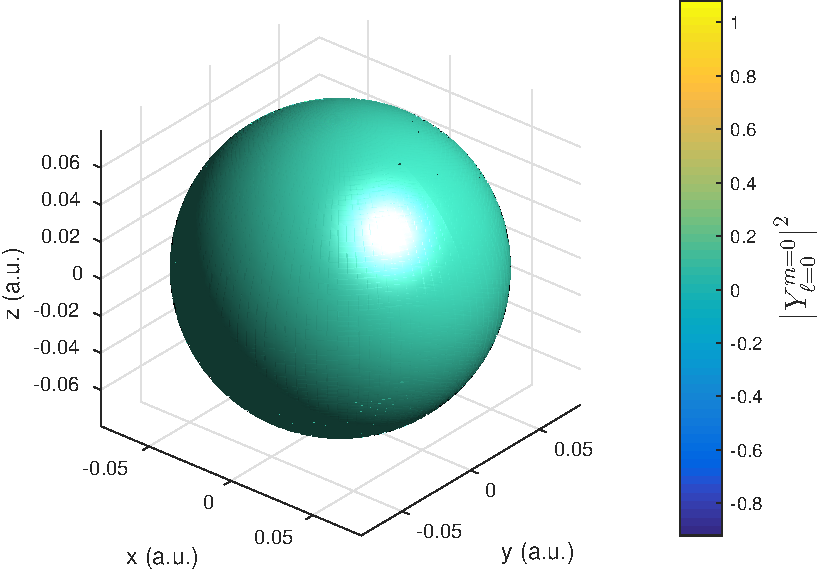
\includegraphics{./Y00.png}
% hw02_03a.pdf: 204x92 pixel, 72dpi, 7.20x3.25 cm, bb=0 0 204 92
 \caption{Y00}
\label{fig:Y00}
\end{figure}

\begin{figure}[H]
\centering
\includegraphics{./Y11.png}
% hw02_03a.pdf: 204x92 pixel, 72dpi, 7.20x3.25 cm, bb=0 0 204 92
 \caption{Y11}
\label{fig:Y11}
\end{figure}

\begin{figure}[H]
\centering
\includegraphics{./Y10.png}
% hw02_03a.pdf: 204x92 pixel, 72dpi, 7.20x3.25 cm, bb=0 0 204 92
 \caption{Y10}
\label{fig:Y10}
\end{figure}



\begin{figure}[H]
\centering
\includegraphics{./Y1-1.png}
% hw02_03a.pdf: 204x92 pixel, 72dpi, 7.20x3.25 cm, bb=0 0 204 92
 \caption{Y1-1}
\label{fig:Y1-1}
\end{figure}

\begin{figure}[H]
\centering
\includegraphics{./Y22.png}
% hw02_03a.pdf: 204x92 pixel, 72dpi, 7.20x3.25 cm, bb=0 0 204 92
 \caption{Y22}
\label{fig:Y22}
\end{figure}

\begin{figure}[H]
\centering
\includegraphics{./Y21.png}
% hw02_03a.pdf: 204x92 pixel, 72dpi, 7.20x3.25 cm, bb=0 0 204 92
 \caption{Y21}
\label{fig:Y21}
\end{figure}

\begin{figure}[H]
\centering
\includegraphics{./Y20.png}
% hw02_03a.pdf: 204x92 pixel, 72dpi, 7.20x3.25 cm, bb=0 0 204 92
 \caption{Y20}
\label{fig:Y20}
\end{figure}

\begin{figure}[H]
\centering
\includegraphics{./Y2-1.png}
% hw02_03a.pdf: 204x92 pixel, 72dpi, 7.20x3.25 cm, bb=0 0 204 92
 \caption{Y2-1}
\label{fig:Y2-1}
\end{figure}

\begin{figure}[H]
\centering
\includegraphics{./Y2-2.png}
% hw02_03a.pdf: 204x92 pixel, 72dpi, 7.20x3.25 cm, bb=0 0 204 92
 \caption{Y2-2}
\label{fig:Y2-2}
\end{figure}




    \end{enumerate}
    
 

\end{homeworkProblem}




\section{Problem 5}

\begin{homeworkProblem}

(5 points) What are the major nuclear data libraries and which countries manage them?

\begin{enumerate}[(a)] 

\item  Briefly describe what each term in the Transport Equation physically
represents.




\subsection{Solution}
    
   
\begin{enumerate}[A)] 

\item Time rate of change of the neutron angular flux, the change in the neutron angular flux for an energy group  over the entire volume, as a function of time.. 

\item Streaming losses, the rate at which neutrons exit the control volume.

\item Total interaction losses, the rate at which neutrons are absorbed or outscattered from an energy and solid angle group.

\item External source gains, the rate at which neutrons enter the system, or from a generic point/line/distributed/etc source (other than fission) in the system.

\item Inscattering source gains, the rate at which neutrons are scattered into an energy and solid angle group.

\item Fission source gain, the rate at which neutrons are born through fission, into a particular energy group.


\end{enumerate}

   
   
\item   Rewrite the time independent form of the equation to include azimuthal
symmetry. Show the steps needed to get there.


\subsection{Solution}
    
   The first step is to make the time-independent assumption:
   
   \begin{equation}
\pderiv{\psi}{t} = 0
\end{equation}

This also removes all time dependence terms:
   
   
   \begin{equation}
\begin{split}
 \omvec\cdot  \nabla \psi(\rvec,E,\omvec) + \Sigma_t(\rvec,E)\psi(\rvec,E,\omvec)  &= S(\rvec, E, \omvec) 
\\
&+\int_0^{\infty}\int_{4\pi}\Sigma_s(\rvec, E'\rightarrow E,\omvec'\rightarrow\omvec) \psi(\rvec,E',\omvec')d\omvec'dE'
\\
& +\frac{\chi_p(E)}{4\pi}\int_0^{\infty}\int_{4\pi}\nu(E')\Sigma_f(\rvec,E') \psi(\rvec,E',\omvec')d\omvec'dE'
\end{split}
\end{equation}

 For the azimuthal symmetry assumption, scattering is only a function of \(\mu =\vOmega' \cdot \vOmega\), the cosine of the scattering angle. This gives us the  simplifications:
 
\(d\vOmega = \sin(\theta) d\theta d\varphi = d\mu d\varphi; \quad \mu = \cos(\theta);$  $d\mu = \sin(\theta)d\theta\:.\)
\begin{align}
\int_{4 \pi} d\vOmega &= \int_0^{2\pi} d\varphi \int_{-\pi/2}^{\pi/2} \sin(\theta) d\theta =  \int_0^{2\pi} d\varphi \int_{-1}^1 d\mu = 4\pi \\
\psi(\rvec,\vOmega,E) d\vOmega &= \psi(\rvec,\varphi, \mu,E) d\varphi  d\mu =  \psi(\rvec, \mu,E) d\varphi  d\mu 
\end{align}

The scattering cross section is no longer dependent on \(\varphi\):

\begin{equation}
\Sigma_s(\rvec, \vOmega' \rightarrow \vOmega) \rightarrow \Sigma_s(\rvec, \vOmega' \cdot \vOmega) = \Sigma_s(\rvec, \mu) 
\end{equation}



Thus,

\begin{equation}
\int_{4 \pi} d\vOmega\: \psi(\rvec, \vOmega, E) =   \int_0^{2\pi} d\varphi \int_{-1}^1 d\mu \:\psi(\rvec, \vOmega, E) = 2 \pi \int_{-1}^1 d\mu \:\psi(\rvec, \mu, E)
\end{equation}

Finally, the fission term can now be written in terms of the scalar flux:

\begin{equation}
\begin{split}
\frac{\chi_p(E)}{4\pi}\int_0^{\infty}\int_{4\pi}\nu(E')\Sigma_f(\rvec,E') \psi(\rvec,E',\omvec')d\omvec'dE' &=
 \frac{\chi_p(E)}{4\pi}\int_0^{\infty}\nu(E')\Sigma_f(\rvec,E') dE'  \int_{4\pi} \psi(\rvec,E',\omvec')d\omvec'
\\
&= \frac{\chi(E)}{2} \int_0^{\infty} dE'\:  \nu(E')\Sigma_f(\rvec,E')\phi(\rvec, E')
\end{split}
\end{equation}

Combining these all together:

 
   \begin{equation}
\begin{split}
 \mu\cdot  \nabla \psi(\rvec,E,\mu) + \Sigma_t(\rvec,E)\psi(\rvec,E,\mu)  &= S(\rvec, E, \mu) 
\\
&+ 2\pi\int_0^{\infty}dE' \int_{-1}^1\Sigma_s(\rvec, E'\rightarrow E,\mu') \psi(\rvec,E',\mu')d\mu'
\\
& +\frac{\chi(E)}{2} \int_0^{\infty} dE'\:  \nu(E')\Sigma_f(\rvec,E')\phi(\rvec, E')
\end{split}
\end{equation}


% \begin{figure}[H]
%  \centering
%  \includegraphics{./hw02_04a.pdf}
%  % hw02_03a.pdf: 204x92 pixel, 72dpi, 7.20x3.25 cm, bb=0 0 204 92
% \end{figure}
% 


    \end{enumerate}
    
 

\end{homeworkProblem}



\end{document}
